\section{System Architecture}
\label{sec:architecture}

The detection system has two stages: a multi-modal encoder mapping raw sensor signals to a latent representation, and an autoregressive decoder reconstructing the G-code token sequence from this representation (Fig.~\ref{fig:architecture}).
The encoder is pre-trained and frozen; only the decoder is trained for reconstruction.
At inference, anomalies are detected by comparing the decoder's reconstruction against the claimed G-code and computing an anomaly score from the discrepancy.

\begin{figure}[t]
    \centering
    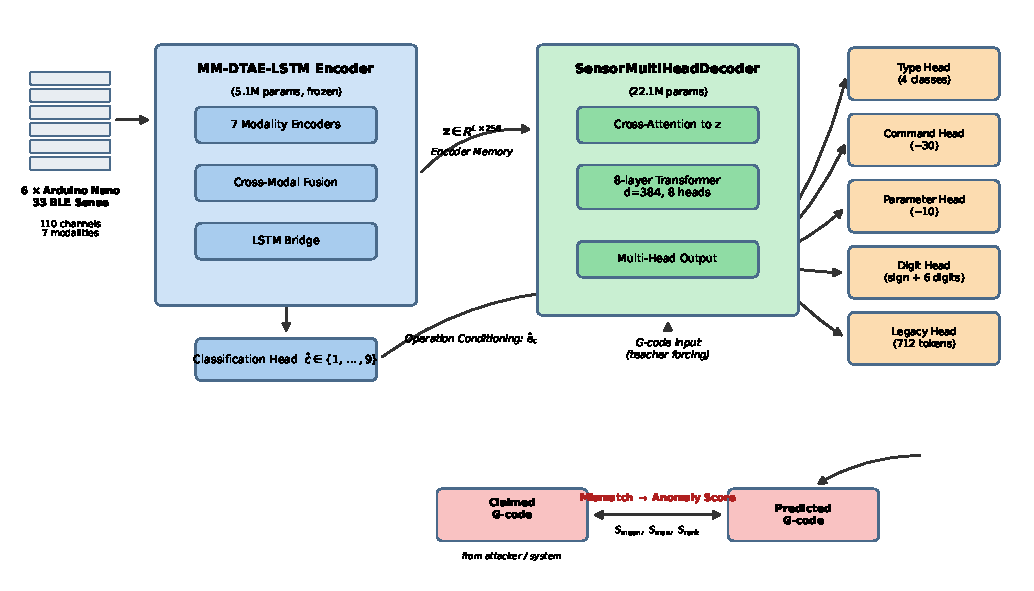
\includegraphics[width=\textwidth]{figures/architecture_overview}
    \caption{System architecture overview. Sensor signals from six Arduino-based boards (110 channels, seven modality groups) are encoded by the frozen MM-DTAE-LSTM encoder into a latent sequence $\mathbf{z}$. The autoregressive SensorMultiHeadDecoder reconstructs the G-code token sequence conditioned on $\mathbf{z}$ and the operation-type embedding. Anomaly scores are computed by comparing the decoder's predicted token distribution against the claimed G-code tokens.}
    \label{fig:architecture}
\end{figure}

\subsection{Encoder: MM-DTAE-LSTM}
\label{sec:encoder}

The encoder is a Multi-Modal Denoising Transformer Autoencoder with LSTM bridge (MM-DTAE-LSTM, 5.1M parameters), developed and validated in prior work where it achieves 100\% operation-type classification accuracy across all 9 classes in 5-fold cross-validation.
For anomaly detection, the encoder is \emph{frozen}: its weights are not updated during decoder training, preventing catastrophic forgetting of the classification capability (used for decoder conditioning) and halving training cost (only 22.1M decoder parameters are optimized rather than the combined 27.2M).

\paragraph{Input representation.}
Six Arduino Nano 33 BLE Sense Lite boards are attached at different positions on the machine structure, providing seven modality groups and 110 input features per time step (the f110 configuration).
Four inertial boards contribute 18 channels each (3-axis accelerometer, gyroscope, magnetometer, and derived features); additional boards provide audio and color sensing (24 channels), environmental measurements (6 channels), and spindle/axis drive currents (8 channels).

Each modality group is processed by a \texttt{LinearModalityEncoder} (linear projection to $d_{\text{model}} = 128$, layer normalization~\cite{ba2016layer}, GELU activation, sinusoidal positional encoding).
A \texttt{CrossModalFusion} module combines modality-specific representations using learned modality gates and cross-attention, with modality dropout ($p = 0.1$) during training to promote robustness to partial sensor failure.

\paragraph{Temporal modeling.}
The fused representation passes through a Transformer encoder with a denoising autoencoder (DTAE) objective that adds Gaussian noise to input embeddings during training, regularizing the representations and providing robustness to MEMS sensor noise.
A bidirectional LSTM bridge captures sequential dynamics, producing the latent sequence $\mathbf{z} = (\mathbf{z}_1, \ldots, \mathbf{z}_L) \in \mathbb{R}^{L \times 128}$ that serves as decoder memory via cross-attention.

\paragraph{Classification head.}
A pooled classification head applied to the mean LSTM output produces the operation-type prediction $\hat{c} \in \{1, \ldots, 9\}$, achieving 100\% test accuracy across all 5 cross-validation folds.
The predicted class label conditions the decoder (Section~\ref{sec:decoder}).

\subsection{Decoder: SensorMultiHeadDecoder}
\label{sec:decoder}

The decoder is a 22.1M-parameter Transformer decoder~\cite{vaswani2017attention} with causal self-attention and cross-attention to $\mathbf{z}$.
Two configurations share the same architecture but differ in maximum sequence length:

\begin{itemize}
    \item \textbf{V7 (short-context)}: \texttt{max\_token\_len} = 6, decoding 3 content tokens per window ($\approx$1 G-code line: command, parameter, value).
    \item \textbf{V8 (multi-line)}: \texttt{max\_token\_len} = 64, decoding up to 63 content tokens spanning multiple G-code lines, providing inter-line sequential context.
\end{itemize}

Both use $d_{\text{model}} = 384$, 8 Transformer layers, 8 attention heads (head dimension 48), $d_{\text{ff}} = 1536$, and dropout $p = 0.1$.

\paragraph{Operation conditioning.}
Because the encoder achieves perfect classification accuracy, the decoder receives the ground-truth operation type as conditioning during both training and inference.
In deployment, if the encoder misclassifies the operation type, the decoder receives incorrect conditioning.
We do not separately evaluate detection under corrupted operation conditioning and flag it as a deployment risk (Section~\ref{sec:limitations}); the leave-one-class-out study (Section~\ref{sec:ablation_loco}) addresses the related but distinct case of detecting entirely novel operation classes.
The operation type is embedded as $\mathbf{e}_c \in \mathbb{R}^{128}$ and added to the encoder memory:
\begin{equation}
    \tilde{\mathbf{z}}_l = \mathbf{z}_l + \mathbf{W}_c \mathbf{e}_c, \quad l = 1, \ldots, L
    \label{eq:op_conditioning}
\end{equation}
where $\mathbf{W}_c \in \mathbb{R}^{128 \times 128}$ is a learned projection.
This conditioning disambiguates sensor signals that are similar across operation types (e.g., similar vibration profiles for face milling and pocket milling at the same feed rate and depth of cut).

\subsection{Multi-Head Output Structure}
\label{sec:multihead}

Rather than a single softmax over the full 712-token vocabulary, the decoder uses a multi-head output structure where each head predicts one G-code token field:

\begin{itemize}
    \item \textbf{Type head} ($|\mathcal{V}_{\text{type}}| = 4$): Predicts token type (command, parameter, numeric, or special), constraining which downstream heads are active.
    \item \textbf{Command head} ($|\mathcal{V}_{\text{cmd}}| \approx 30$): Predicts the G/M code (e.g., G0, G1, G2, G3, M3, M5, M6, M30).
    \item \textbf{Parameter head} ($|\mathcal{V}_{\text{param}}| \approx 10$): Predicts the parameter letter (X, Y, Z, F, S, R, I, J, K).
    \item \textbf{Sign-and-digit head}: A \texttt{DigitByDigitValueHead} predicting numeric values one digit at a time (sign, up to 4 integer digits, up to 4 decimal digits).
    \item \textbf{Legacy head} ($|\mathcal{V}| = 712$): Full-vocabulary softmax providing the primary probability distribution for anomaly scoring.
\end{itemize}

The digit-by-digit decomposition avoids the combinatorial explosion of discretizing continuous axis values into fixed bins.
This structured output enables fine-grained anomaly attribution (command substitution elevates command-head error; coordinate perturbation elevates digit-head error) and provides natural grammar constraints: inconsistencies between type predictions and downstream heads constitute trivially detectable grammar violations.

\paragraph{Grammar and type constraint masks.}
During inference, precomputed masks enforce structural constraints.
A type constraint mask $\mathbf{M}_{\text{type}} \in \{0, 1\}^{4 \times 712}$ restricts the legacy head's softmax to tokens valid for the predicted type.
A grammar constraint mask $\mathbf{M}_{\text{grammar}} \in \{0, 1\}^{712 \times 712}$ encodes valid token transitions (e.g., G1 can be followed by X, Y, Z, or F, but not another G command).
Both masks are derived from the G-code grammar specification, not learned.

\subsection{Training}
\label{sec:training}

The decoder is trained with the encoder frozen, using a multi-task loss summing cross-entropy across all active heads:
\begin{equation}
    \mathcal{L}_{\text{decoder}} = \sum_{h \in \mathcal{H}} \lambda_h \sum_{t=1}^{T} -\log p_h(y_t^{(h)} \mid y_{<t}, \tilde{\mathbf{z}})
    \label{eq:decoder_loss}
\end{equation}
where $\mathcal{H} = \{\text{type}, \text{cmd}, \text{param}, \text{digit}, \text{legacy}\}$, $\lambda_h = 1.0$ for all heads, $y_t^{(h)}$ is the ground-truth token for head $h$ at position $t$, and $\tilde{\mathbf{z}}$ is the operation-conditioned encoder memory (Eq.~\ref{eq:op_conditioning}).
Label smoothing ($\epsilon = 0.1$) and focal loss ($\gamma = 2.0$) are applied to improve calibration and focus on hard examples.
Training uses AdamW~\cite{loshchilov2019decoupled} ($\text{lr} = 3 \times 10^{-4}$, weight decay $10^{-2}$, cosine annealing with 5-epoch warmup, gradient clipping at norm 1.0, batch size 32).
V7 converges in $\sim$50 epochs ($\sim$2 hours/fold on an RTX A6000); V8 requires $\sim$80 epochs ($\sim$4 hours/fold).
